\documentclass{article}

\usepackage[margin=1in]{geometry}
\usepackage{amsmath}
\usepackage{float}
\usepackage{amsfonts}
\usepackage{graphicx}

\author{\begin{tabular}{l@{\hspace{2em}}r}Zachary \textsc{Vogel}& Maurice \textsc{Woods} III\end{tabular}\\[1.5ex]
\begin{tabular}{l@{\hspace{1.5em}}r}Derek \textsc{Reamon} & Mechatronics\end{tabular}
}
\date{\today}
\title{\textbf{\begin{tabular}{c}Grad Project Equations in MCEN 5115:\\Rotating Inverted Pendulum\end{tabular}}}

\begin{document}
\maketitle

\section*{Normal Inverted Pendulum}
\begin{figure}[H]
    \centering
    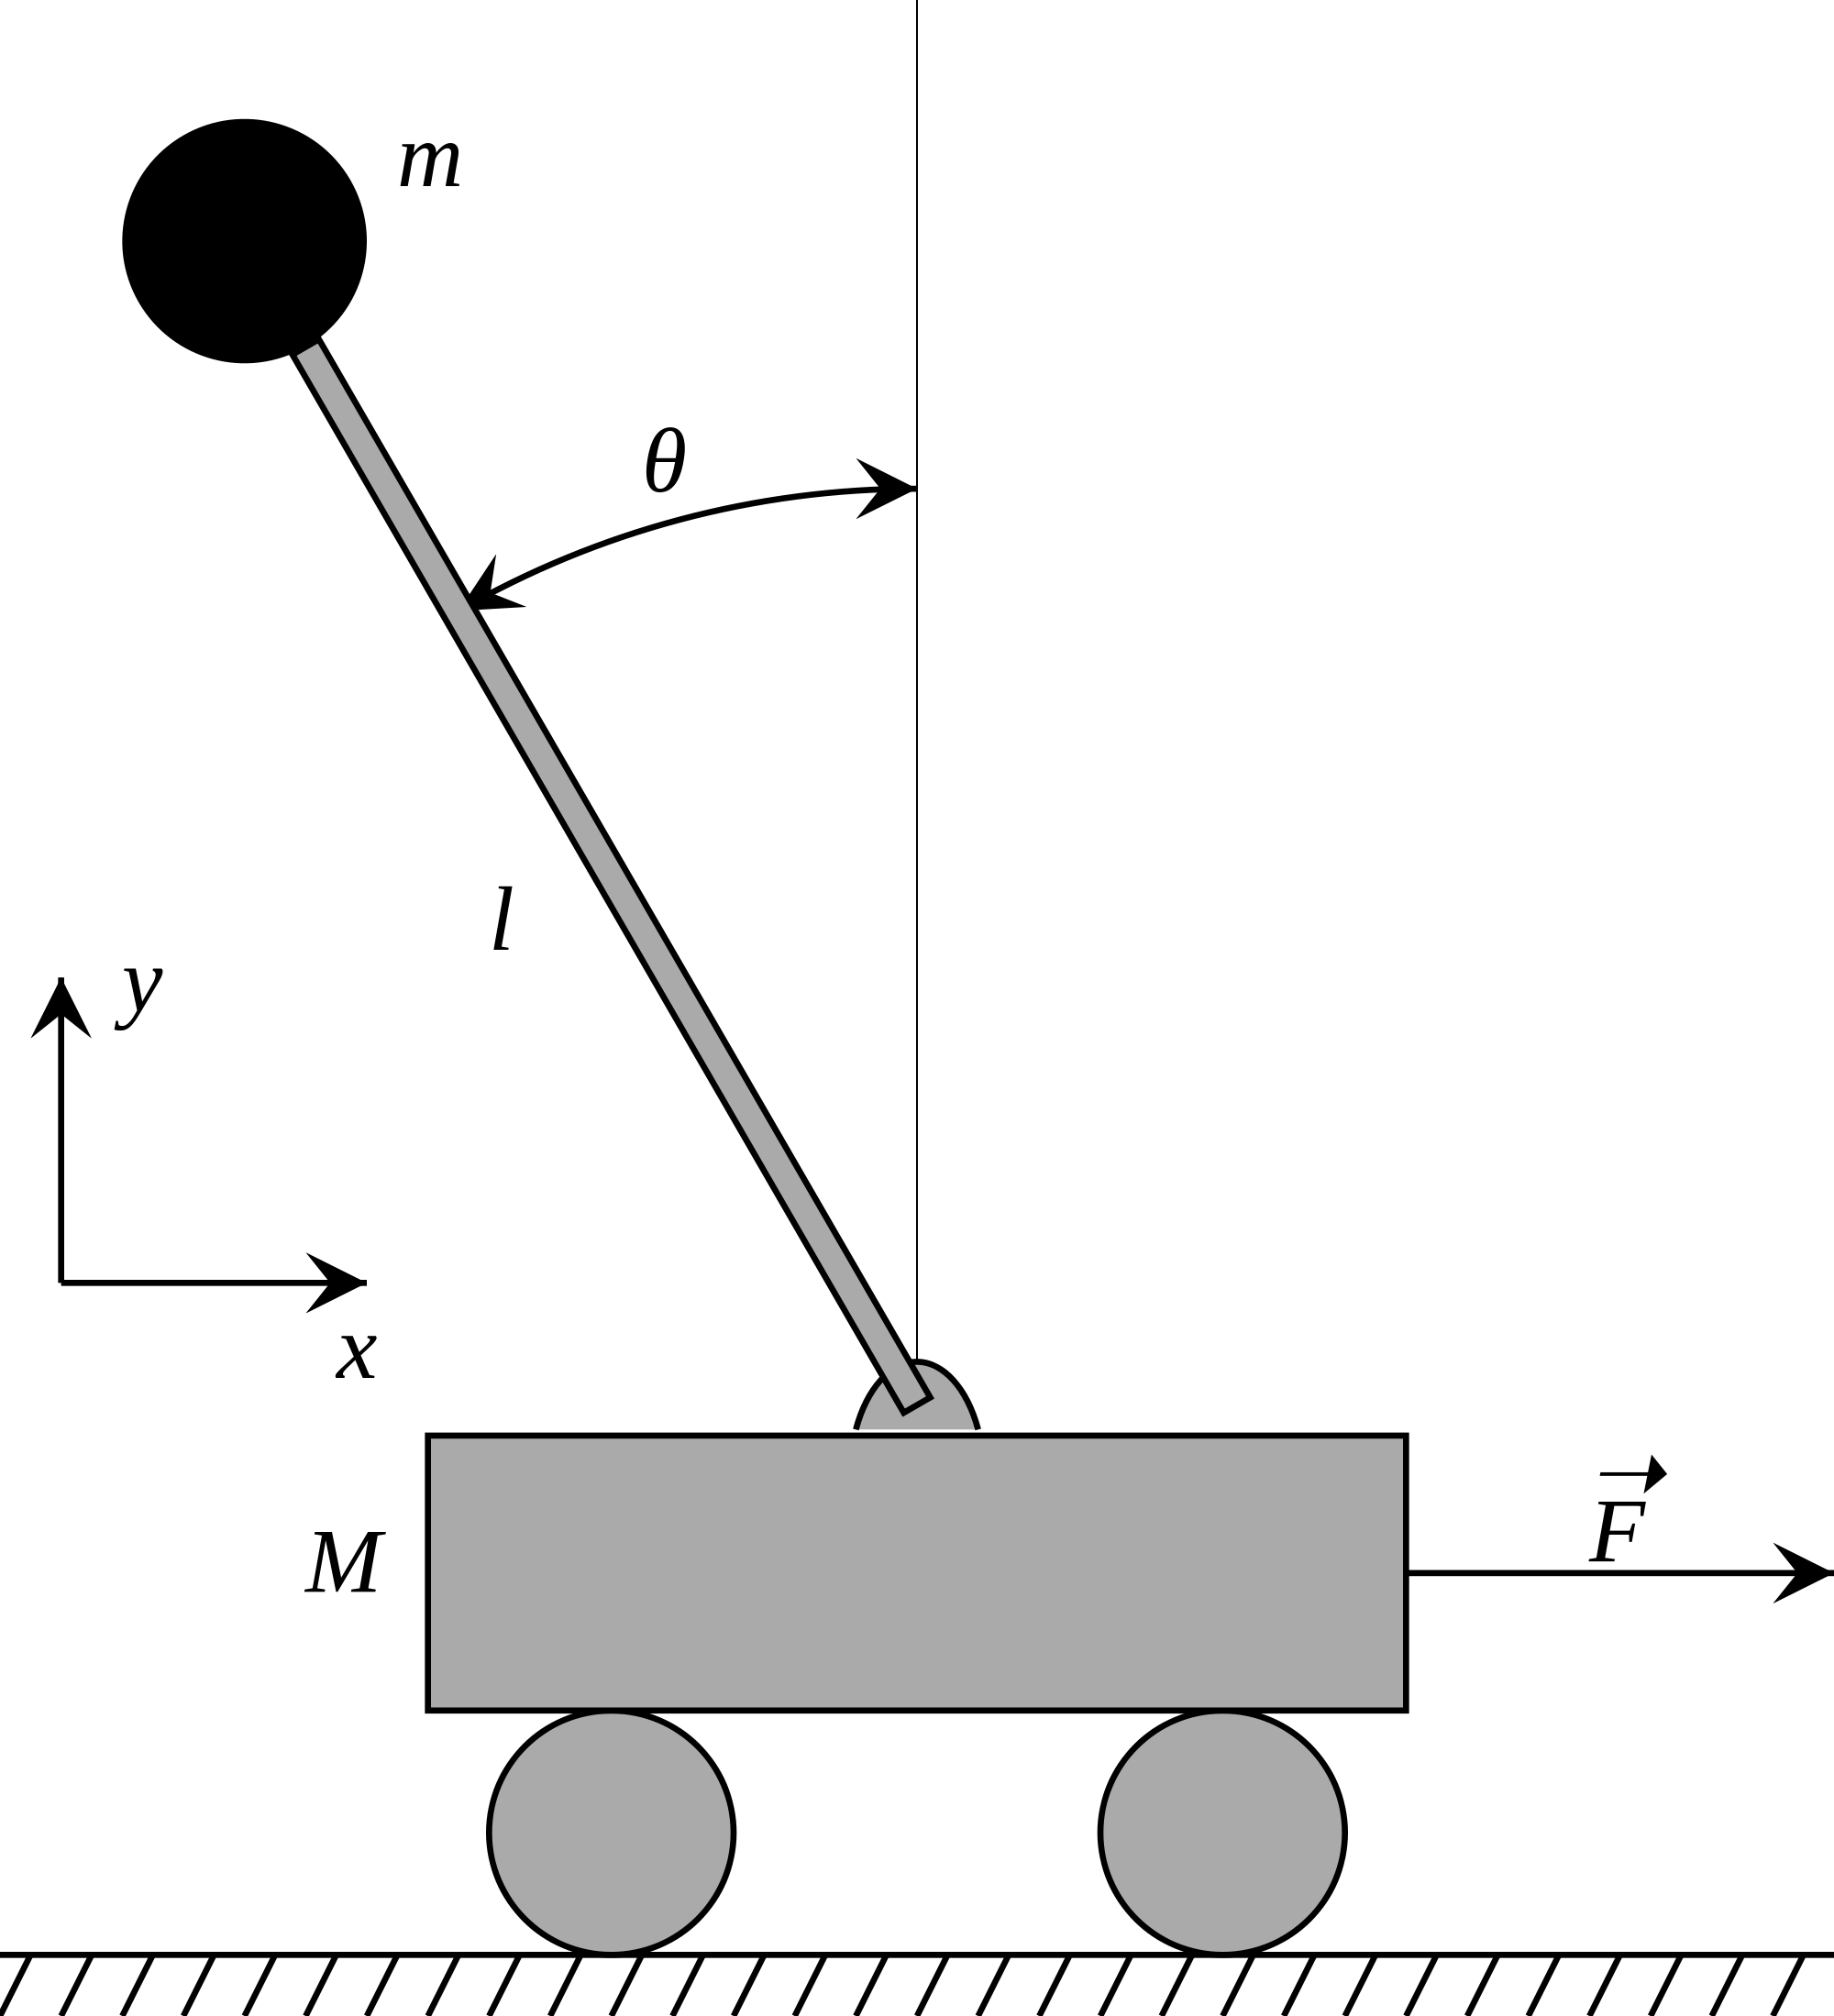
\includegraphics[width=0.7\textwidth]{inv_pend.png}
    \caption{sup sup}
\end{figure}
Here we have the normal inverted pendulum equations for the image above:
\[\begin{split}(M+m)\ddot{x}-ml\ddot{\theta}+ml(\dot{\theta})^2\sin(\theta)=F\\l\ddot{\theta}-g\sin(\theta)=\ddot{x}\cos(\theta)\end{split}\]
The $x$ position for us is actually $\omega$ because we are spinning. Also, the input force isn't $F$. What we have is a torque $\tau=\lvert\lvert r\rvert\rvert\lvert\lvert F\rvert\rvert\sin(\theta)$. Given that the $\theta$ here is 90 degrees or 270 degrees, force can be equated to $F=\frac{\tau}{r}$.\\
Torque is some function of the motor current and the motor properties that we can put in later. We also note that $x=\omega*r$ and thus $\ddot{x}=\ddot{\omega}r$.\\
Thus our equations become:
\[\begin{split}\cfrac{\tau}{r}=ml(\dot{\theta})^2\sin(\theta)-ml\ddot{\theta}+(M+m)\ddot{\omega}r\\\ddot{\omega}r\cos(\theta)=l\ddot{\theta}-g\sin(\theta)\end{split}\]
rewriting with $\ddot{\omega}r=\frac{l\ddot{\theta}-g\sin(\theta)}{\cos(\theta)}$
\[\cfrac{\tau}{r}=ml(\dot{\theta})^2\sin(\theta)-ml\ddot{\theta}+\cfrac{(M+m)(l\ddot{\theta}-g\sin(\theta))}{\cos(\theta)}\]
\[=ml(\dot{\theta})^2\sin(\theta)+\ddot{\theta}\cfrac{((M+m)l-ml\cos(\theta))}{\cos(\theta)}-\cfrac{(M+m)g\sin(\theta)}{\cos(\theta)}\]
\[\ddot{\theta}=\cfrac{\cos(\theta)}{(M+m)l-ml\cos(\theta)}\left (\cfrac{\tau}{r}-ml(\dot{\theta})^2\sin(\theta)-\cfrac{(M+m)g\sin(\theta)}{\cos(\theta)}\right )\]

hmmm, those equations suck to take partial derivatives.
\[\begin{split}\ddot{\theta}=\dot{\theta}^2\sin(\theta)-\cfrac{\tau}{rml}+\cfrac{(M+m)\ddot{\omega}r}{ml}\\\ddot{\omega}=\cfrac{l\ddot{\theta}-g\sin(\theta)}{r\cos(\theta)}\end{split}\]
Now let's pick some variables. $x_1=\dot{\theta}$, $x_2=\theta$, $x_3=\dot{\omega}$ and $x_4=\omega$. We need to linearize around $\omega=0$ and $\dot{\omega}=0$.\\
State matrix will look like:
\[\dot{x}=Ax=\begin{bmatrix}a_0&a_1&a_2&a_3\\1&0&0&0\\b_1&b_2&b_3&b_4\\0&0&1&0\end{bmatrix}\begin{bmatrix}x_1\\x_2\\x_3\\x_4\end{bmatrix}\]
Here we have $a_0=0$, $a_1=\frac{(M+m)g}{(M+m)l-ml}$, $a_2=0$, and $a_3=0$. Now we write out the equations in the other form.\\
\[l\ddot{\theta}=\cfrac{-\tau}{rm}+l(\dot{\theta})^2\sin(\theta)+\cfrac{(M+m)\ddot{\omega}r}{m}\]
this gives:
\[\ddot{\omega}r\cos(\theta)=-\cfrac{\tau}{rm}+l(\dot{\theta})^2\sin(\theta)+\cfrac{(M+m)\ddot{\omega}r}{m}-g\sin(\theta)\]
Simplifying we get:
\[\ddot{\omega}\left(r\cos(\theta)-\cfrac{(M+m)r}{m}\right )=\cfrac{-\tau}{rm}+l(\dot{\theta})^2\sin(\theta)-g\sin(\theta)\]
etc:
\[\ddot{\omega}=\cfrac{-\tau}{r^2(m\cos(\theta)-(M+m))}+\cfrac{ml(\dot{\theta})^2\sin(\theta)}{r(\cos(\theta)-(M+m))}-\cfrac{mg\sin(\theta)}{r(\cos(\theta)-(M+m))}\]
\section*{small angle}
This is not wrong, but we will be doing the small angle approximation then the jacobian. I don't need to do jacobian I need to do small angle approximation. For small $\theta$ $\cos(\theta)\approx 1$ and $\sin(\theta)\approx \theta$ Thus we get:
\[\ddot{\theta}=\cfrac{1}{Ml}\left (\cfrac{\tau}{r}-ml(\dot{\theta})^2\theta-(M+m)g\theta\right )\]
and:
\[\ddot{\omega}=\cfrac{-\tau}{-r^2M}+\cfrac{ml(\dot{\theta})^2\theta}{r(1-(M+m))}-\cfrac{mg\theta}{r(1-(M+m))}\]

Our state equations are thus:
\[\begin{bmatrix}\ddot{\theta}\\\dot{\theta}\\\ddot{\omega}\\\dot{\omega}\end{bmatrix}=\begin{bmatrix}0&-(M+m)g&0&0\\[0.5em]1&0&0&0\\0&\cfrac{-mg}{r(1-(M+m))}&0&0\\[0.5em]0&0&1&0\end{bmatrix}\begin{bmatrix}\dot{\theta}\\\theta\\\dot{\omega}\\\omega\end{bmatrix}+\begin{bmatrix}\cfrac{1}{Mlr}\\[0.5em]0\\\cfrac{1}{r^2M}\\[0.5em]0\end{bmatrix}\tau\]
The output is then:
\[y=\begin{bmatrix}0&1&0&0\end{bmatrix}\begin{bmatrix}\dot{\theta}\\\theta\\\dot{\omega}\\\omega\end{bmatrix}\]

Note here that $a_0$ and $b_1$ are zero. If this doesn't turn out to be good enough we can take the third part of the taylor series for the $\dot{\theta}^2\theta$ term which will be non-zero unlike the first 2.\\
\end{document}
